% ---------------------------------------------------------------------------
% BODY of the paper, \input by the wrapper www2027.tex (ACM sigconf, WWW 2027;
% the Overleaf main document). Edit the text HERE; the wrapper carries only the
% preamble, title, abstract and bibliography. Keep it format-neutral: no
% \usepackage, no \bibliography.
%
% 2026-10-13: restructured as a full paper (intro / related / task / dataset /
% framework / experiments / discussion). Every number is measured: the slice
% rows under the final prompt configuration (11 §10.3h/j), the core set (10.3i).
% Numbers marked \pend{...} are runs in flight (held-out set, test slice, VERITAS,
% frontier) and are to be filled in before submission.
% ---------------------------------------------------------------------------
\newcommand{\pend}[1]{\textit{#1}}
\newcommand{\sys}{\textsc{MedTempo-Hypo}}

\begin{figure*}[t]
\centering
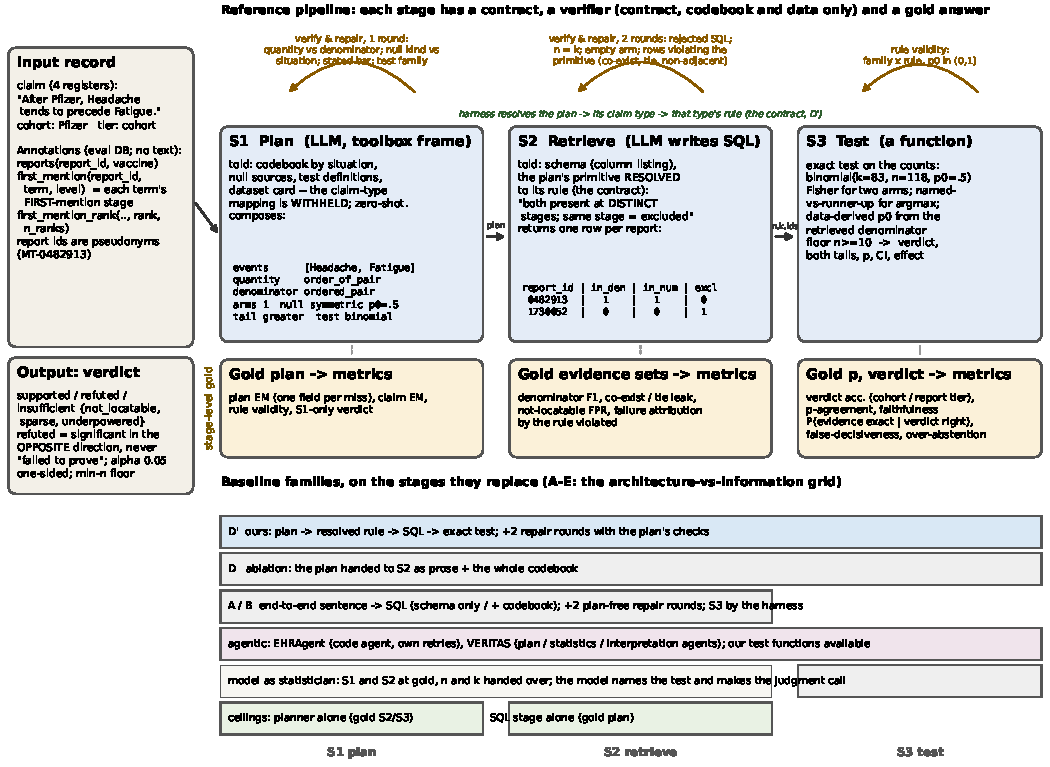
\includegraphics[width=\textwidth]{Figures/overview.pdf}
\caption{Overview. A claim about annotated adverse-event timelines (left) is
verified by a three-stage reference pipeline (centre): S1 composes a
\emph{plan} from stated conventions, with the claim-type mapping withheld; the
harness resolves the plan's named denominator primitive into its definition and
S2 writes the retrieval query under that contract; S3 runs the exact test.
Each stage has a bounded verify-and-repair loop and a gold answer, so the stage
metrics beneath (plan EM; denominator F1, co-exist leak; $p$-agreement,
faithfulness, abstention) are measured in addition to the verdict. Baseline
families (bottom) are placed on the stages they replace: end-to-end
sentence-to-SQL with and without the conventions and with plan-free repair,
agentic systems, and counts-given judgment.}
\label{fig:overview}
\end{figure*}

\section{Introduction}
\label{sec:intro}

A growing class of language-model systems promises to test scientific
hypotheses against data: given a claim and a dataset, they choose a statistical
method, run it and report a conclusion. Benchmarks for this ability
\cite{miao2026fisher,zhu2024statqa,zhu2026statabench} score the final answer ---
a $p$-value, a reject/fail-to-reject decision --- and hand the system the
relevant data already assembled. In most real settings that is the easy half.
Consider the claim \emph{``after the Pfizer vaccine, headache tends to precede
fatigue''} against a corpus of annotated adverse-event reports. Before any test
can run, a system has to decide \emph{which reports count}: those in which both
events occur at different stages (a report where they co-occur witnesses
neither order), \emph{what ``no effect'' means} (a 50/50 split of the ordered
reports), and \emph{which test applies} (a one-sided exact binomial with a
minimum-count floor). Each of those decisions is a stipulation about what the
sentence means for this corpus, each can be wrong independently of the others,
and a verdict can be right while all of them are wrong.

This paper makes that chain of decisions the object of evaluation. We release
\sys{}, a benchmark of temporal--statistical claims over MedTempo, a corpus of
3{,}166 vaccine adverse-event reports whose clinical course is annotated as a
\emph{leveled order} of events. Every instance carries not only its gold
verdict --- \emph{supported}, \emph{refuted} or \emph{insufficient}, the last
sub-typed --- but the gold of every stage that produced it: the structured plan
(events, quantity, denominator rule, null, test), the exact set of report
identifiers in the denominator and numerator, and the exact $p$-values. Gold is
computed mechanically from the annotations, validated by six families of
invariants, and reproduced to 1.000 by a deterministic oracle, so a system's
intermediate outputs can be scored, not only its answer.

We pair the benchmark with an \emph{instrumented reference pipeline}: a plan
stage, a retrieval stage and a deterministic test stage, each with an explicit
output contract and a bounded verify-and-repair loop. The pipeline is a
measuring instrument as much as a method: its stages can be filled with gold,
its prompts can state or withhold the corpus conventions, and its plan can be
handed to the next stage either as prose or as a contract that the harness
resolves. That lets us separate two things that end-to-end evaluation
conflates --- the \emph{information} a system is told and the
\emph{architecture} it is given --- and ask what each is worth.

Three findings organise the results. First, \emph{the denominator is where
systems fail, and verdict accuracy hides it}: the strongest end-to-end
text-to-SQL baseline is right 59\% of the time but stands on the correct
evidence for only 28\% of its right answers; an agentic baseline reaches 0.62
on the cohort tiers while deciding 64\% of the claims the data cannot decide.
Second, \emph{stated conventions are worth as much as any architecture}: one
missing stipulation cost a 32B planner a whole claim family (0 of 18) and the
sentence that supplied it moved the planner from 0.897 to 0.950 with 23 of 26
groups unchanged record for record. Third, \emph{decomposition pays only when
the plan is a contract}: with the plan handed to retrieval as prose, the
pipeline with a verifier is matched by a verified end-to-end model (0.645 vs.\
0.660); with the plan resolved by the harness it reaches 0.865 on the
development slice and 0.856 on the 2{,}350-instance development set, 0.19 above
the verified end-to-end control, while being right for the right reason 78\%
of the time against 53\%.

Our contributions are: (i) a benchmark of 8{,}763 claim instances
(70{,}104 renderings) in 26 groups and seven claim families over three cohort
tiers, with stage-level gold, exact-test labels, a three-decision verdict with
sub-typed abstention, pseudonymised identifiers and declared splits
(\S\ref{sec:dataset}); (ii) an evaluation framework whose stage contracts turn
the verdict into five auditable quantities --- plan agreement, evidence-set
agreement, $p$-agreement, faithfulness and abstention --- and whose prompt
frames make information and architecture separately controllable
(\S\ref{sec:framework}); (iii) an experimental study of local and agentic
systems under that framework, including a one-change-at-a-time account of what
the conventions, the schema presentation and the plan contract are each worth
(\S\ref{sec:experiments}).

\section{Related Work}
\label{sec:related}

\paragraph{Statistical reasoning benchmarks.} StatQA \cite{zhu2024statqa}
scores whether a model knows which test applies; StatFormBench
\cite{wang2026statformbench} scores the formulation of a test family from a
description; StatABench \cite{zhu2026statabench} adds fixed tool functions and
scores the final answer. P-Bench and Fisher-R1 \cite{miao2026fisher} come
closest to our setting: 425 tasks in which an agent receives a hypothesis with
its null stated, a CSV of the relevant data and a glossary, writes R to compute
a $p$-value, and is scored on the decision and on the $p$-value's distance to
a reference. In all of these the data are already the relevant subset and the
null is given or trivial. The step we score first --- deciding which records a
statistic is computed over --- has no counterpart, and no intermediate stage
has gold.

\paragraph{Hypothesis-testing agents.} VERITAS \cite{veritas2026} is a
multi-agent co-scientist that formulates, analyses and interprets a hypothesis
with a deterministic evidence classifier, built for image-derived cohorts; LATCH
\cite{gim2026latch} runs LLM-chosen analyses through deterministic R pipelines
on EHR data with the method given; DiscoveryBench and BLADE
\cite{majumder2025discoverybench,gu2024blade} evaluate open-ended data-driven
discovery agents against rubrics. These systems share our plan-then-execute
shape and our insistence on auditable computation; none of them scores the
conditioning of the evidence, and none has hypotheses about the order of
events within a record. We run two of them (EHRAgent \cite{shi2024ehragent},
VERITAS) on our data as end-to-end baselines.

\paragraph{Clinical text-to-SQL and timelines.} EHRSQL \cite{lee2022ehrsql}
scores one query per question with an abstention option; EHRAgent
\cite{shi2024ehragent} solves EHR questions with a code-writing agent and
error-driven retries. The sentence-to-SQL baselines in \S\ref{sec:baselines}
follow that protocol over our schema. MedTempo and the CRAFT/TIMER line
\cite{craft2026,timer2025} extract clinical timelines from narratives; we start
where extraction ends, taking the expert-annotated timelines as given and
asking what can be claimed about them.

\paragraph{Positioning.} Table~\ref{tab:related} compares the closest work on
the dimensions that decide what can be claimed. Two things are not new: a
plan-then-execute loop with a deterministic statistics layer is the LATCH
architecture, and ``hypothesis and data in, method and $p$ out'' is P-Bench.
What is new is the combination of a model-formulated null executed
deterministically with gold at every stage, a scored eligibility rule, and
claims about event order with the conditioning semantics (first mention,
co-existence, ties) those claims carry.

\begin{table*}[t]
\centering
\scriptsize
\setlength{\tabcolsep}{3pt}
\renewcommand{\arraystretch}{1.15}
\begin{tabularx}{\textwidth}{@{}p{2.55cm} Y Y Y Y Y Y@{}}
\toprule
Work & Formulates the null? & Statistic computed by & Event-order claims & Clinical & Gold at intermediate stages & Dataset-in interface \\
\midrule
P-Bench / Fisher-R1 \cite{miao2026fisher} & no; $H_0$ given, test chosen but unscored & model-written R in a sandbox & no (survival only) & partly & no; final $p$ and decision & no; 425 fixed tasks \\
LATCH \cite{gim2026latch} & no; hypothesis and method both given & deterministic R pipelines & no (cross-sectional) & yes (NHANES) & partial; cohort $n$, CI vs.\ the paper & yes; schema summary \\
StatFormBench \cite{wang2026statformbench} & family label only & nothing computed & no & textbook & formulation only & no \\
StatABench \cite{zhu2026statabench} & test selection, no null & fixed tool functions & no & no & final answer & no \\
StatQA \cite{zhu2024statqa} & applicability only & nothing computed & no & no & final answer & no \\
DiscoveryBench / BLADE \cite{majumder2025discoverybench,gu2024blade} & open-ended hypothesis & agent code & no & no & rubric / expert & no \\
EHRAgent / EHRSQL \cite{shi2024ehragent,lee2022ehrsql} & no (QA / SQL) & agent code / SQL & no & yes (EHR) & answer / execution & schema \\
VERITAS \cite{veritas2026} & plans the analysis & own code + deterministic classifier & no & yes (imaging) & verdict vs.\ reference & data + description \\
CRAFT / TIMER \cite{craft2026,timer2025} & n/a (extraction) & n/a & timelines, no claims & yes & reference timeline & n/a \\
\midrule
\textbf{This work} & \textbf{yes}: null recipe (kind, $p_0$ or how to compute it, reference population), denominator, test family + rule & \textbf{deterministic harness} runs the stated rule; exact tests & \textbf{yes}: precedes, co-occur, sequence, first/last, position, proximity, threshold & \textbf{yes}: annotated VAERS timelines & \textbf{every stage}: plan, evidence set, counts, $p$, verdict & stated conventions + dataset card \\
\bottomrule
\end{tabularx}
\caption{Positioning against the closest benchmarks and systems. ``Gold at
intermediate stages'' is what makes per-stage attribution possible;
``event-order claims'' means hypotheses about the order or timing of events
within a record.}
\label{tab:related}
\end{table*}

\section{Task}
\label{sec:task}

\paragraph{Input and output.} A \emph{record} is a claim in natural language
--- a question or a declarative sentence, in one of four registers --- about a
\emph{cohort} (the reports of one vaccine), a \emph{contrast} of two cohorts, or
one named \emph{report}; and the annotations: for every report, its vaccine
and the stage at which each event term is first mentioned. The system must
return a verdict in $\{\emph{supported}, \emph{refuted}, \emph{insufficient}\}$,
the last sub-typed as \emph{not-locatable} (no report qualifies),
\emph{sparse} (too few qualify) or \emph{underpowered} (enough qualify, neither
tail significant). It never sees report text.

\paragraph{What a verdict rests on.} For a cohort-tier claim the gold is
computed in three steps that are themselves released: (1) a \emph{plan} ---
the events named, the quantity compared, the \emph{denominator primitive}
(which reports count), the number of arms, the null (a fixed proportion, a bar
stated in the text, a rate derived from the data, or equality of two arms), the
tail and the test family; (2) the \emph{evidence} --- the identifiers of the
reports in each arm's denominator and numerator; (3) the exact test with a
per-family minimum-count floor and $\alpha = 0.05$ one-sided in the claim's
direction. \emph{Refuted} requires significance in the opposite direction, never
``failed to prove''. A report-tier claim is a single deterministic observation
over one report and carries no test.

\paragraph{Conventions are part of the task.} Whether a report with both
events at the same stage counts for ``precedes'', what ``typically'' means,
whether a tie for ``first'' leaves the denominator, what ``more often than their
separate rates would predict'' compares --- these are stipulations about the
corpus, not facts about the sentence, and a system that was never told them
cannot infer them. The benchmark therefore ships its conventions as a
situation-phrased text that any system may be given (\S\ref{sec:frames}), and
the experiments treat ``conventions stated'' as a controlled condition. The
claim-type \emph{mapping} --- which rule and which test go with which wording
--- is what we withhold: a system is scored on composing it.

\paragraph{Metrics.} Verdict accuracy and class-macro F1 are reported on the
cohort tiers (the statistical headline) and on the report tier (a reading
task) separately. Because every stage has gold, we also report plan agreement
(exact match on the plan's fields), denominator-set F1 and the \emph{co-exist
leak} (same-stage reports wrongly admitted to an order denominator),
$p$-agreement with the exact computation, \emph{faithfulness} --- the share of
correct verdicts whose denominator is exactly the gold set --- and three
abstention measures: false-decisiveness (a decisive verdict on a gold
\emph{insufficient} claim), over-abstention and sub-type accuracy.

\section{The \sys{} Benchmark}
\label{sec:dataset}

\subsection{Source corpus}
\label{sec:corpus}

MedTempo is a corpus of 3{,}166 VAERS adverse-event reports for three COVID-19
vaccines, annotated with a \emph{leveled order}: a single totally ordered chain
of stages in which each stage holds the MedDRA-coded events reported at that
point of the clinical course (Table~\ref{tab:corpus}). Two annotation
conventions are load-bearing: when a term recurs, its \emph{first} mention
fixes its stage; events at one stage are temporally indistinguishable
(\emph{co-exist}). The annotation, not the narrative, is both the benchmark's
ground truth and the systems' input.

\begin{table}[t]
\centering
\small
\begin{tabular}{lr}
\toprule
Reports & 3{,}166 \\
\quad Janssen / Pfizer / Moderna & 1{,}164 / 1{,}019 / 983 \\
Distinct event terms (vocabulary) & 1{,}660 \\
Events per report (mean / median / max) & 7.2 / 6 / 43 \\
Stages per report (mean / median / max) & 3.4 / 3 / 14 \\
\bottomrule
\end{tabular}
\caption{Source corpus. Stages are the levels of the annotated leveled order.}
\label{tab:corpus}
\end{table}

\subsection{Hypothesis space}
\label{sec:space}

Twenty-nine template groups span seven claim families at three scopes
(Table~\ref{tab:roster}). Four families concern order and co-occurrence ---
\emph{precedes}, \emph{co-occurs}, strict \emph{sequence} of three events,
\emph{first/last} among candidates --- and three, added to diversify the null,
concern \emph{position} (an event in the earlier half of a timeline),
\emph{proximity} (two events at consecutive stages) and \emph{threshold} (a
rate at least a stated bar). Scopes are a single report, one vaccine cohort,
and a contrast of two cohorts. Within a cohort, three groups are two-arm
contrasts: whether $B$ follows $A$ more often than it follows $C$; whether $A$
precedes $B$ more often than $C$ precedes $D$; and whether $A$ and $B$ occur
together more often than their separate rates predict (association). Each
group is realised in four registers (a canonical \textsc{Original} plus
\textsc{Research}, \textsc{Media} and \textsc{Clinical}) and two formats
(question and claim) by mechanical slot-filling with no model-generated
rewriting; answers are \textsc{Bool} or \textsc{Choice}.

\begin{table}[t]
\centering
\small
\begin{tabular}{llll}
\toprule
Family & Report & One cohort & Two cohorts \\
\midrule
precedes & P-R1, P-R2 & P-V1--P-V4 & P-M2 \\
co-occurs & C-R1 & C-V1--C-V3 & --- \\
sequence & S-R1 & --- & --- \\
first/last & F-R1--F-R3 & F-V1--F-V3 & --- \\
position & T-R1 & T-V1 & --- \\
proximity & Y-R1 & Y-V1--Y-V3 & --- \\
threshold & --- & H-V1, H-V5 & --- \\
\bottomrule
\end{tabular}
\caption{The 26-group roster: 9 report-level, 16 single-cohort, 1 two-cohort.}
\label{tab:roster}
\end{table}

\paragraph{Five kinds of null.} Order claims test a proportion against the
symmetry value $0.5$; argmax claims (``most common first'', ``most common
ordering'') test the named cell against its strongest competitor; two-arm
claims test the equality of two rates; threshold claims read their null off
the text (``in at least two thirds''); and the position and proximity-rate
claims use a null \emph{derived from the data} --- the structural early-rate of
the denominator reports, or the chance $2/L$ that two events of an $L$-stage
report are adjacent --- which no lookup table can supply. The last two kinds
are what make ``formulate the null'' a scored capability rather than a
classification.

\subsection{Gold labels}
\label{sec:gold}

\paragraph{Conditioning.} Each family fixes its denominator, and these
distinctions are the substantive content of the task. \emph{Precedes} counts
only reports where both events occupy distinct stages. \emph{Co-occurs} counts
all reports containing both, because co-existence is the event of interest.
\emph{Sequence} requires all three events at distinct stages. \emph{First/last}
requires every candidate present and drops tie reports entirely. Association
conditions on presence alone, comparing $P(B \mid A)$ against $P(B \mid \neg
A)$ over the whole cohort. \emph{Immediate} order counts reports where the two
events are at consecutive occupied stages; \emph{position} drops single-stage
reports and events on the exact middle stage.

\paragraph{Tests.} All tests are exact. Majority and bar claims use a one-sided
exact binomial against $p_0$; argmax claims use modal-versus-runner-up, an exact
binomial on the named cell against its strongest competitor; two-arm and
two-cohort contrasts use Fisher's exact test. No $\chi^2$ approximation
appears; the sole gate is a per-family minimum denominator ($n \geq 10$;
sequence $n \geq 5$), applied to both arms where two exist.

\paragraph{The three-decision rule and oriented statistics.} A claim is
\emph{supported} only when its own one-sided tail is significant at
$\alpha = 0.05$, \emph{refuted} only when the opposite tail is, and otherwise
\emph{insufficient} (\emph{underpowered}, \emph{sparse}: $0 < n <$ floor, or
\emph{not-locatable}: $n = 0$). Both tails are computed for every instance.
Every released statistic --- both $p$-values, the Wilson interval, Cohen's $h$
against the null actually used --- describes the claim as that instance asserts
it.

\subsection{Instance realisation and composition}
\label{sec:realization}

Every decisive core is posed \emph{both ways}: oriented with its effect
(\emph{supported}) and against it (\emph{refuted}), a mirror pair over
identical evidence, so a system answering \emph{supported} to both directions
of one fact is caught immediately. Direction-asking groups re-orient by
swapping slots; symmetric claims re-orient by authored negation, written into
the template rather than derived; threshold claims are tested per orientation
(both directions can be refuted) and carry no mirror. Each cohort group ships
equal thirds --- supported, refuted, insufficient --- balanced \emph{per group}
because template wording is fixed per group and a skewed group would teach a
text-shape-to-label shortcut; the insufficient third is spread over its
sub-types. \emph{Not-locatable} instances are minted deliberately from real
cohort vocabulary whose joint count is zero, so the claim appears answerable and
only querying the annotations reveals the empty denominator. Groups are capped
at 600 instances (200 per class) by a seeded draw that keeps mirror pairs
together; report groups ship two classes of 200.

\subsection{Validity screens}
\label{sec:screens}

No group ships on plausibility. Each is screened against a permutation null
matched to its claim shape at 2{,}000 rounds: a \emph{level shuffle}
(term-to-stage assignment permuted within each report, preserving report size,
stage-size multiset, term frequencies and co-occurrence) for order, position
and proximity groups; a degree-preserving \emph{edge swap} for association; a
\emph{label shuffle} for two-cohort contrasts (Table~\ref{tab:screens}). The
screening history is itself a result: seven candidate two-cohort shapes were
tested and one survived; a majority statistic was replaced after the screen
showed its text and its test answered different questions; and a rank-test
track was retired when the Mann--Whitney approximation proved anti-conservative
on tie-heavy ordinal data (${\sim}11\%$ of cores decisive under shuffled labels
at a nominal 5\%).

\begin{table}[t]
\centering
\small
\setlength{\tabcolsep}{4pt}
\begin{tabular}{llrrr}
\toprule
Group & Null & Decisive & Null mean $\pm$ sd & $p_{\textrm{perm}}$ \\
\midrule
P-V4 & level shuffle & 16{,}884 & 1{,}848.9 & $<$0.0005 \\
P-V2 & level shuffle & 2{,}302 & 341.3 & $<$0.0005 \\
C-V3 & level shuffle & 258 & 62.6 & $<$0.0005 \\
C-V2 & edge swap & 2{,}098 & 924.4 & $<$0.0005 \\
P-M2 & label shuffle & 30 & 18.3 & 0.025 \\
Y-V1/Y-V2 & level shuffle & 68 & 14.9 $\pm$ 3.8 & $<$0.0005 \\
Y-V3 & level shuffle & 35 & 15.5 $\pm$ 3.8 & $<$0.0005 \\
T-V1 & level shuffle & 34 & 4.4 $\pm$ 2.0 & $<$0.0005 \\
H-V1 & level shuffle & 402 & 351.3 $\pm$ 9.4 & $<$0.0005 \\
H-V5 & level shuffle & 228 & 196.9 $\pm$ 10.3 & 0.002 \\
\bottomrule
\end{tabular}
\caption{Permutation screens at 2{,}000 rounds (0.0005 is the resolution
floor). ``Decisive'' is the group's decisive-core supply at its shipping
universe; for the threshold groups the supported count is the screened
statistic, since a bar claim can be refuted by chance in either direction.}
\label{tab:screens}
\end{table}

\subsection{Release, splits and leakage}
\label{sec:release}

\paragraph{Two files.} The questions file carries one row per rendering and
only the input fields (identifier, group, level, answer type, register, format,
text, options, cohort); the answers file carries one row per instance with the
gold verdict and sub-type, the oriented counts, both $p$-values, the test, the
floor, interval and effect size, and the \emph{evidence identifiers}. The writer
refuses to emit a gold field into the questions file. A group-independent
\texttt{fact\_id} keys every split, because answer-format twins pose the same
fact under two groups.

\paragraph{Pseudonymised identifiers.} Every report identifier a system can
see --- in the claim texts, in the released evidence and in the database --- is
a keyed permutation of the public VAERS identifier. VAERS is public and in
pretraining corpora; removing the lookup key removes the shortcut without
touching the annotations.

\paragraph{Splits.} The release declares a \emph{development set} of 2{,}350
instances (a seeded, class-balanced draw of at most 90 per group, mirror pairs
and facts kept together) and a \emph{test set} of 1{,}742 instances drawn by the
same recipe from the remainder, fact-disjoint from the development set. Each
contains a 200-instance \emph{budget subset} stratified over groups for
systems whose cost is paid per call. All prompt and design decisions in this
paper were made on the development subset; the test set was run once.

\paragraph{Validation.} Six families of mechanical invariants --- evidence
arithmetic, set algebra, per-family conditioning re-derived from the leveled
orders, direction, verdict-against-tails including the floor, and independent
recomputation through a separate database path --- are checked over the whole
enumerated universe (56{,}138 instances). A deterministic oracle (reverse
template parser into the reference SQL compiler) reproduces every gold label of
the release: the harness is correct, whatever the text entails.

\subsection{Statistics}
\label{sec:stats}

Tables~\ref{tab:totals} and~\ref{tab:pergroup} summarise the release. The
earlier, uncapped version of the benchmark let one group contribute 46\% of all
instances; the cap makes the eleven largest groups equal in size, and
class balance is exact within every cohort group by construction.

\begin{table}[t]
\centering
\small
\begin{tabular}{lr}
\toprule
Records (instance $\times$ register $\times$ format) & 70{,}104 \\
Instances & 8{,}763 \\
Groups / families / tiers & 26 / 7 / 3 \\
Distinct cores & 5{,}703 \\
Distinct facts (split key) & 4{,}761 \\
\midrule
Supported / refuted / insufficient & 3{,}521 / 3{,}521 / 1{,}721 \\
\quad underpowered / sparse / not-locatable & 605 / 498 / 618 \\
Mirror pairs & 3{,}060 \\
Negated instances & 643 \\
\midrule
Conditioned $n$, median (IQR) & 21 (14--41) \\
$|$Cohen's $h|$ on decisive, median & 0.65 \\
$p$ on supported claims, median & 0.008 \\
\bottomrule
\end{tabular}
\caption{Aggregate statistics of the release.}
\label{tab:totals}
\end{table}

\begin{table*}[t]
\centering
\scriptsize
\setlength{\tabcolsep}{3.5pt}
\begin{tabular}{llllrrrrrlrr}
\toprule
Group & Sc. & Claim & Ans. & Null & Inst. & Sup. & Ref. & Insuf. & u/s/n & Facts & Med.\ $n$ \\
\midrule
P-R1 & R & precedes & \textsc{Boo} & --- & 400 & 200 & 200 & 0 & --- & 200 & --- \\
P-R2 & R & precedes & \textsc{Cho} & --- & 400 & 200 & 200 & 0 & --- & 200 & --- \\
C-R1 & R & co-occur & \textsc{Boo} & --- & 400 & 200 & 200 & 0 & --- & 400 & --- \\
S-R1 & R & sequence & \textsc{Boo} & --- & 400 & 200 & 200 & 0 & --- & 200 & --- \\
F-R1 & R & first & \textsc{Cho} & --- & 400 & 200 & 200 & 0 & --- & 200 & --- \\
F-R2 & R & last & \textsc{Cho} & --- & 400 & 200 & 200 & 0 & --- & 200 & --- \\
F-R3 & R & first & \textsc{Boo} & --- & 400 & 200 & 200 & 0 & --- & 200 & --- \\
T-R1 & R & early half & \textsc{Boo} & --- & 400 & 200 & 200 & 0 & --- & 400 & --- \\
Y-R1 & R & immediately before & \textsc{Boo} & --- & 400 & 200 & 200 & 0 & --- & 200 & --- \\
\midrule
P-V1 & C & precedes & \textsc{Boo} & sym.\ 0.5 & 501 & 167 & 167 & 167 & 55/56/56 & 334 & 17 \\
P-V3 & C & precedes & \textsc{Cho} & sym.\ 0.5 & 501 & 167 & 167 & 167 & 55/56/56 & 334 & 17 \\
P-V2 & C & antecedent contrast & \textsc{Boo} & two-arm & 600 & 200 & 200 & 200 & 66/67/67 & 375 & 22 \\
P-V4 & C & pair-vs-pair contrast & \textsc{Boo} & two-arm & 600 & 200 & 200 & 200 & 66/67/67 & 393 & 24 \\
C-V1 & C & co-occur majority & \textsc{Boo} & sym.\ 0.5 & 600 & 200 & 200 & 200 & 66/67/67 & 400 & 19 \\
C-V2 & C & association & \textsc{Boo} & two-arm & 600 & 200 & 200 & 200 & 100/0/100 & 400 & 229 \\
C-V3 & C & co-occur argmax & \textsc{Boo} & runner-up & 522 & 174 & 174 & 174 & 58/58/58 & 348 & 23 \\
F-V1 & C & first argmax & \textsc{Cho} & runner-up & 102 & 34 & 34 & 34 & 11/11/12 & 68 & 14 \\
F-V2 & C & last argmax & \textsc{Cho} & runner-up & 138 & 46 & 46 & 46 & 15/15/16 & 92 & 14 \\
F-V3 & C & first argmax & \textsc{Boo} & runner-up & 102 & 34 & 34 & 34 & 11/11/12 & 68 & 14 \\
T-V1 & C & early half vs.\ structural rate & \textsc{Boo} & data-derived & 102 & 34 & 34 & 34 & 19/0/15 & 68 & 145 \\
Y-V1 & C & immediate order & \textsc{Boo} & sym.\ 0.5 & 204 & 68 & 68 & 68 & 22/23/23 & 136 & 17 \\
Y-V2 & C & immediate order & \textsc{Cho} & sym.\ 0.5 & 204 & 68 & 68 & 68 & 22/23/23 & 136 & 17 \\
Y-V3 & C & adjacency vs.\ $2/L$ & \textsc{Boo} & data-derived & 105 & 35 & 35 & 35 & 11/12/12 & 70 & 26 \\
H-V1 & C & precedes $\geq 2/3$ & \textsc{Boo} & text 0.667 & 105 & 35 & 35 & 35 & 11/12/12 & 101 & 16 \\
H-V5 & C & first $\geq 1/2$ & \textsc{Boo} & text 0.5 & 66 & 22 & 22 & 22 & 7/7/8 & 61 & 13.5 \\
\midrule
P-M2 & M & precedes, 2 cohorts & \textsc{Boo} & two-arm & 87 & 29 & 29 & 29 & 9/10/10 & 58 & 21.5 \\
\bottomrule
\end{tabular}
\caption{Per-group composition. Scope: R = report, C = one cohort, M = two
cohorts. Null: sym.\ = symmetric $0.5$; runner-up = named cell vs.\ strongest
competitor; two-arm = equality of two rates; text = bar read off the wording;
data-derived = computed from the denominator reports. u/s/n gives the
insufficient sub-types (underpowered / sparse / not-locatable); Facts counts
distinct \texttt{fact\_id}; median $n$ is the conditioned denominator.}
\label{tab:pergroup}
\end{table*}

\section{Evaluation Framework}
\label{sec:framework}

\subsection{Stage contracts}
\label{sec:contracts}

The reference pipeline decomposes verification into three stages with explicit
output contracts (Figure~\ref{fig:overview}).

\textbf{S1 --- plan.} From the record (text, level, cohort) the model composes
a plan: \texttt{events}, \texttt{quantity}, \texttt{denominator} (a named
primitive: \emph{ordered\_pair}, \emph{both\_present},
\emph{all\_present\_unique\_first}, \emph{consecutive\_pair},
\emph{present\_offmid}, \emph{presence\_split}, \emph{single\_report}, \ldots),
\texttt{arms}, \texttt{null\_kind} with $p_0$ or a reference population,
\texttt{tail}, \texttt{test\_family} and a rule for the floor. The harness
derives the claim type from the plan by reverse lookup over the plan's fields;
a plan that names no known shape is \emph{underdetermined} and scored as
insufficient. Two normalisation folds are applied before lookup: a
consecutive-pair denominator implies the immediate-order quantity, and a
stated or derived null on a shape with no such twin keeps the shape and costs
one field.

\textbf{S2 --- retrieve.} For each arm the model writes one SQL statement over
the annotation database (two tables, two views) that returns \emph{one row per
report} with four flags: in the denominator, in the numerator, excluded, and an
optional cell label for argmax claims. The harness executes it in a read-only
sandbox and aggregates the rows into $(n, k)$ per arm together with the
identifier sets, so the evidence is auditable against the gold sets.

\textbf{S3 --- test.} A deterministic function runs the plan's test on the
counts: the exact binomial against the plan's $p_0$ (for a data-derived null,
against the chance sum over the retrieved denominator), Fisher's test for two
arms, modal-versus-runner-up for argmax; applies the floor; and returns the
verdict with both tails. Nothing is inferred at S3.

\subsection{Information: what the model is told}
\label{sec:frames}

The S1 prompt comes in two frames. The \emph{catalogue} frame hands the model
the table of claim types with their conditioning rule, null and test, so
planning reduces to classification and lookup; it is an answer-injected upper
bound. The \emph{toolbox} frame withholds that mapping and states every
convention by situation --- ``a report with two events tied for earliest has no
answer and is excluded''; ``order words are distance-blind; only wording that
says the two are adjacent conditions on consecutive stages''; ``association
wording compares the rate of $B$ among reports with $A$ against reports without
$A$'' --- together with a computed dataset card, the null sources and the test
definitions, and the model composes the plan. Zero-shot is the headline
condition: a worked plan is a mapping row.

The S2 prompt is where the plan is handed over, and it can be handed over in
two ways. As \emph{prose}: the plan's JSON and the full conventions text, from
which the SQL model must work out what the named primitive means. As a
\emph{contract}: the harness resolves the plan's claim type and supplies that
type's conditioning rule and arm plan in the prompt --- the same stipulation,
stated once, for the one primitive the plan names. The second is the
pipeline's design; the first is the ablation that shows why.

\subsection{Verification}
\label{sec:verify}

Each stage has a bounded verify-and-repair loop that reads only the contract,
the stated conventions and the data --- never the gold. At S1 the plan is
checked for consistency with the conventions (a quantity against its
denominator, a null kind against its situation, a stated bar against the
wording, a valid test family) and re-asked once with the violations named. At
S2 a statement that the database rejects, an arm whose denominator equals its
numerator, an empty arm beside a full one, and --- when a plan exists --- rows
that violate the plan's primitive (co-existing reports in an order
denominator, ties in a first/last denominator, non-consecutive pairs in an
immediate denominator) trigger a re-ask, up to two rounds. The end-to-end
baselines receive the same loop with the checks that need no plan, which is
the control for what verification is worth without a contract. The planner
alone settles after one round; the SQL stage after two.

\subsection{Baselines}
\label{sec:baselines}

\emph{Sentence-to-SQL} (cells A and B): the same SQL model writes the
per-report rows directly from the sentence, given the schema only (A) or the
schema and the conventions (B); S3 is the harness's. \emph{Agentic}: EHRAgent
\cite{shi2024ehragent}, a code-writing agent with error-driven retries over the
same database, in a variant that returns counts to our test and one that runs
its own test; VERITAS \cite{veritas2026}, run through its hypothesis,
statistics and interpretation agents with imaging bypassed, given our exact-test
functions and, in one condition, the conventions. \emph{Counts-given judgment}:
the model receives the gold counts and must name the test and the verdict ---
not a competitor but the floor of ``the model does the statistics itself''.
\emph{Ceilings}: the planner alone (gold S2/S3) and the SQL stage alone (gold
plan). Chance on the three-class cohort tiers is $\approx 0.33$; a per-group
majority guesser scores at most 0.37.

\section{Experiments}
\label{sec:experiments}

\subsection{Setup}

Local models are Qwen2.5-32B-Instruct for planning and Qwen2.5-Coder-32B for
SQL (7B variants for the small-model floor), served locally; agentic baselines
use Coder-32B. All rows use the \textsc{Original} register in both formats
(200 instances $=$ 400 records; 258 cohort-tier records), blind to the group
label and with the procedure unspecified, under one frozen prompt
configuration (conventions v2.2, schema shown as column listings, one
self-join hint in the row contract; \S\ref{sec:ablations}). The main table
reports the development budget subset, on which every system can be run, and
the test budget subset; our rows and the end-to-end rows are also run on the
full development set (2{,}350 instances) and the test set (1{,}742).
Every verdict accuracy is reported with a 95\% bootstrap interval over
instances (1{,}000 resamples; an instance's renderings move together). On the
200-instance subset the interval is about $\pm 0.05$ at 0.85 and $\pm 0.06$
at 0.6, so differences under 0.06 between rows are not resolved there; the
full sets resolve 0.02.

\subsection{Main results}
\label{sec:main}

\begin{table*}[t]
\centering
\small
\setlength{\tabcolsep}{4pt}
\begin{tabular}{llrrrrrrr}
\toprule
 & & \multicolumn{2}{c}{verdict acc.} & & & & & \\
system (32B) & verifier & all & cohort & den.\ F1 & co-exist leak & faithfulness & false-dec. & test slice \\
\midrule
\multicolumn{9}{@{}l}{\textit{stage ceilings}} \\
planner alone (gold S2/S3) & 1 round & 0.955 & 0.930 & 0.954 & 0.00 & --- & 0.03 & \pend{pending} \\
SQL stage alone (gold plan) & 2 rounds & 0.905 & 0.853 & 0.803 & 0.16 & 0.79 & 0.00 & \pend{pending} \\
\midrule
\multicolumn{9}{@{}l}{\textit{ours: plan as contract}} \\
D$'$ & none & 0.855 & 0.775 & 0.717 & 0.15 & 0.75 & 0.01 & \pend{pending} \\
\textbf{D$'$ + verifier} & 2 rounds & \textbf{0.865} & \textbf{0.791} & \textbf{0.763} & 0.16 & \textbf{0.78} & \textbf{0.00} & \pend{pending} \\
\midrule
\multicolumn{9}{@{}l}{\textit{end-to-end sentence $\rightarrow$ SQL, same model and S3}} \\
A: schema only & none & 0.502 & 0.562 & 0.441 & 0.60 & 0.21 & 0.10 & \pend{pending} \\
B: + conventions & none & 0.588 & 0.543 & 0.517 & 0.47 & 0.28 & 0.18 & \pend{pending} \\
\midrule
\multicolumn{9}{@{}l}{\textit{agentic}} \\
EHRAgent, counts $\rightarrow$ our test, + conventions & own retries & --- & 0.628 & n/a & n/a & n/a & 0.23 & 0.58 \\
EHRAgent, runs its own test & own retries & 0.743 & 0.624 & n/a & n/a & n/a & 0.64 & 0.63 \\
VERITAS + conventions, our tests (claim form, 129 cohort claims) & own critic & --- & 0.349 & n/a & n/a & n/a & 0.19 & 0.317 \\
\midrule
counts-given judgment (gold $n,k$) & --- & 0.705 & 0.543 & (given) & --- & 1.00 & 0.17 & \pend{pending} \\
\bottomrule
\end{tabular}
\caption{Main results on the development budget subset (200 instances, 400
records; cohort $=$ 258 cohort-tier records) under the frozen configuration.
Den.\ F1 is the denominator-set F1 over cohort arms; faithfulness is
$P(\text{denominator exact} \mid \text{verdict right})$; false-dec.\ is the
share of gold-\emph{insufficient} claims given a decisive verdict. EHRAgent's
evidence cannot be audited (it returns counts or a verdict, not report sets);
its report-tier accuracy (0.96) carries its overall number. VERITAS takes the
claim form only; 50 of its 129 runs completed all three phases within a
10-minute cap per phase (the rest are scored as misses), and the completed
runs abstain on 29 of 36 undecidable claims but on 69 of 93 decisive ones. The last column is
the same row's cohort-tier accuracy on the test budget subset (EHRAgent: 240
cohort-tier records; its own-test variant scores 0.743 overall there too).}
\label{tab:main}
\end{table*}

Table~\ref{tab:main} reports every system on the same 400 records. Three
observations carry the paper.

\paragraph{The denominator is where systems fail, and the verdict hides it.}
The best end-to-end baseline (B + repair) is right on 66\% of records; on the
cohort tiers it is within 0.01 of our pipeline without the verifier. But its
right answers stand on the exact gold evidence only 53\% of the time, it admits
same-stage reports into order denominators on 56\% of its arms, and it gives a
decisive verdict to 15\% of the claims the data cannot decide. The agentic
baseline that runs its own test reaches 0.743 overall --- mostly on the
report tier (0.96) --- and 0.624 on the cohort tiers while deciding 64\% of the
undecidable claims; the multi-agent VERITAS, given the same conventions and our
tests, completes 39\% of its runs and scores 0.349, abstaining on most decisive
claims --- the opposite failure. Verdict accuracy ranks these systems within a few points of
each other; the evidence metrics do not.

\paragraph{Each stage is nearly solved alone; the hand-off is the loss.} The
planner alone scores 0.955 with one repair round and the SQL stage alone 0.905
with the gold plan, so the composed product should be near 0.86. Handing the
plan to the SQL stage as prose gives 0.573 (Table~\ref{tab:grid}); resolving
it as a contract gives 0.855, and 0.865 with the verifier --- within 0.04 of
the gold-plan ceiling. The remaining gap is the planner's own errors.

\paragraph{Verification without a contract has little to check.} The end-to-end
model gains $+0.07$ from two repair rounds, almost all of it from statements
that previously failed to execute; the conditioning errors remain, because
nothing in a sentence-to-SQL system states which reports its query should have
excluded. The same rounds on our pipeline check the rows against the plan's
primitive and remove most of the co-exist and tie leaks
(Table~\ref{tab:attribution}).

\subsection{Scale and generalisation}
\label{sec:scale}

\begin{table}[t]
\centering
\small
\setlength{\tabcolsep}{3.5pt}
\begin{tabular}{lrrrrrr}
\toprule
 & \multicolumn{3}{c}{development set (2{,}350)} & \multicolumn{3}{c}{test set (1{,}742)} \\
system (32B) & all & cohort & faith. & all & cohort & faith. \\
\midrule
planner alone, 1 round & 0.954 & 0.931 & --- & \pend{---} & \pend{---} & --- \\
SQL stage alone, 2 rounds & 0.880 & 0.816 & 0.81 & \pend{---} & \pend{---} & \pend{---} \\
D$'$ & 0.831 & 0.743 & 0.75 & \pend{---} & \pend{---} & \pend{---} \\
\textbf{D$'$ + verifier} & \textbf{0.856} & \textbf{0.781} & \textbf{0.78} & \pend{---} & \pend{---} & \pend{---} \\
A: schema only & 0.466 & 0.494 & 0.21 & \pend{---} & \pend{---} & \pend{---} \\
B: + conventions & 0.590 & 0.525 & 0.32 & \pend{---} & \pend{---} & \pend{---} \\
counts-given judgment & 0.739 & 0.602 & 1.00 & \pend{---} & \pend{---} & --- \\
\bottomrule
\end{tabular}
\caption{The same rows on the full development set (3{,}080 cohort-tier
records) and on the fact-disjoint test set, which no prompt decision was made
on.}
\label{tab:scale}
\end{table}

The development-subset numbers hold on the full development set within 0.03
(Table~\ref{tab:scale}): D$'$ with the verifier 0.856, the verified end-to-end
control 0.669, the planner 0.954. Because every prompt decision was made on the
development subset, the test set is the honest check of those decisions; its
numbers are \pend{pending at the time of writing}.

\paragraph{Frontier and open-weight models.} The same rows, prompts and
flags with Claude Opus~5.5 and GPT-5.6 in every model slot
(Table~\ref{tab:frontier}) put the development subset within reach of a
frontier model with no contract at all: end-to-end with the conventions
stated they score 1.000 and 0.995 with every denominator exact, and the
contract pipeline 0.990 and 0.995. The two models agree to within one record
on every row. The newest open-weight generation, run with thinking off on one
workstation GPU, closes most of that distance \emph{with} the contract:
gemma4-31B reaches 0.970 and qwen3.8-27B 0.905 with the verifier, against
0.925 and 0.895 for the verified end-to-end control. The contract's verdict
margin therefore shrinks as models improve, from $+0.155$ at the Qwen2.5-32B
pair to $+0.045$ at gemma4 and within the interval at qwen3.8; its
faithfulness margin does not: with the contract 96\% of right verdicts rest on
the exact denominator for both models, against 81--89\% end-to-end, and
false-decisiveness halves. The statements are right for the right reason
--- the precedes arm, for instance, excludes same-level reports from the
denominator and flags them as such --- so the stipulations, stated once, are
sufficient information for a model that can hold them. Without them
(cell~A) the same models score 0.945 and 0.925 and get 79--83\% of
denominators exactly: they infer most of the stipulations from the schema and
the wording, and the stated conventions close the rest. Each column cost
under \$9 at list price with prompt caching, about 20~minutes per row.
What the contract buys, then, is not accuracy a frontier model lacks but
accuracy an open 32B model lacks (0.87 against 0.66--0.72 end-to-end at zero
API cost) and a verdict whose denominator can be audited; and the test set,
which no prompt decision was made on, is where frontier difficulty has to be
measured.

\begin{table*}[t]
\centering
\small
\begin{tabular}{lrrrrr}
\toprule
system, development subset (200 claims) & Opus 5.5 & GPT-5.6 & gemma4-31B & qwen3.8-27B & Qwen2.5-32B \\
\midrule
planner alone (S2, S3 at gold) & 0.990 & 0.995 & 0.985 & 0.945 & 0.965 \\
D$'$ & 0.990 & 0.995 & 0.890 & 0.845 & 0.865 \\
D$'$ + verifier & 0.990 & 0.990 & \textbf{0.970} & \textbf{0.905} & \textbf{0.870} \\
A: schema only & 0.945 & 0.925 & --- & --- & 0.505 \\
B: + conventions & \textbf{1.000} & \textbf{0.995} & 0.875 & 0.840 & 0.640 \\
counts-given judgment & 1.000 & 1.000 & 0.810 & 0.700 & 0.705 \\
\midrule
denominator F1, D$'$ + verifier & 1.000 & 0.992 & 0.965 & 0.898 & 0.763 \\
faithfulness, D$'$ + verifier & --- & --- & 0.96 & 0.96 & 0.78 \\
\bottomrule
\end{tabular}
\caption{Two frontier models and three open-weight models in every model slot,
same prompts; claim form, original register. Open-weight models run with
thinking off on one RTX A5000. Each frontier column cost under \$9 at list
price with prompt caching. Intervals: $\pm 0.02$ at 0.97, $\pm 0.04$ at 0.90,
$\pm 0.06$ at 0.65.}
\label{tab:frontier}
\end{table*}

\paragraph{Cost and latency.} Table~\ref{tab:cost} gives, per record of the
development subset, the wall time of the sequential harness, the tokens
exchanged and the dollar cost from the providers' own usage counts at list
price with prompt caching; local rows cost GPU time only. The contract
pipeline makes two calls per record where the end-to-end baseline makes one,
so it exchanges about twice the tokens; the repair rounds add 10--20\% on top.
At the frontier a full 200-claim row costs two to three dollars; a local
27B model answers a record in 9~s and a 31B one in 13~s on one workstation
GPU, with the verifier adding four to five seconds.

\begin{table}[t]
\centering
\small
\setlength{\tabcolsep}{4pt}
\begin{tabular}{llrrr}
\toprule
system & model & s / record & tokens / record & USD / record \\
\midrule
D$'$ & Opus 5.5 & 6.0 & 8{,}940 & 0.0125 \\
D$'$ & GPT-5.6 & 5.1 & 5{,}470 & 0.0100 \\
D$'$ & Qwen2.5-32B pair & \pend{x} & 8{,}720 & 0 \\
D$'$ & qwen3.8-27B & 8.8 & 5{,}020 & 0 \\
D$'$ & gemma4-31B & 13.2 & 5{,}130 & 0 \\
B & Opus 5.5 & 4.6 & 4{,}600 & 0.0107 \\
B & GPT-5.6 & 5.5 & 2{,}980 & 0.0094 \\
B & Qwen2.5-Coder-32B & \pend{x} & 3{,}960 & 0 \\
B & gemma4-31B & 4.7 & 2{,}950 & 0 \\
B & qwen3.8-27B & 4.6 & 2{,}890 & 0 \\
counts-given & Opus 5.5 & 2.8 & 930 & 0.0040 \\
counts-given & GPT-5.6 & 9.1 & 980 & 0.0125 \\
\bottomrule
\end{tabular}
\caption{Cost and latency per record on the development subset (claim form).
Tokens are prompt plus visible completion; GPT-5.6's hidden reasoning tokens
are billed but not shown (60 per record on D$'$, 525 on counts-given). Local
latencies are measured on one RTX A5000 with the model fully resident.}
\label{tab:cost}
\end{table}

\subsection{Stage analysis}
\label{sec:stages}

\paragraph{Planning without the mapping.} Table~\ref{tab:toolbox} compares the
two S1 frames. With the catalogue, a 32B model scores 0.998: given the mapping,
planning is lookup. With the mapping withheld the same model composes the plan
at 0.950 zero-shot and 0.955 with one repair round; the 7B model falls to
0.595, almost entirely whole-shape misreads, while the fields that do land are
right. Paraphrase is a bounded perturbation for the capable model
(Table~\ref{tab:registers}): $-0.02$ to $-0.12$ across registers, largest on
the research register, where the wording rewrites the statistical situation
rather than the event names.

\begin{table}[t]
\centering
\small
\begin{tabular}{lrrrr}
\toprule
 & \multicolumn{2}{c}{\textbf{32B-Inst.}} & \multicolumn{2}{c}{7B-Inst.} \\
S1 condition (S2, S3 at gold) & all & cohort & all & cohort \\
\midrule
Catalogue (answer-injected upper bound) & 0.998 & 0.996 & --- & --- \\
\textbf{Toolbox, zero-shot} & 0.950 & 0.922 & 0.595 & 0.558 \\
\quad + one verify-and-repair round & \textbf{0.955} & \textbf{0.930} & 0.657 & 0.655 \\
\bottomrule
\end{tabular}
\caption{Planning with the claim-type mapping given (catalogue) and withheld
(toolbox); development subset; report tier 1.000 at 32B.}
\label{tab:toolbox}
\end{table}

\begin{table}[t]
\centering
\small
\begin{tabular}{lrrrr}
\toprule
 & Original & Research & Media & Clinical \\
\midrule
\multicolumn{5}{l}{\textit{Planner alone (S2, S3 at gold), one round}} \\
7B-Instruct & 0.657 & 0.662 & 0.595 & 0.575 \\
32B-Instruct & 0.955 & 0.838 & 0.877 & 0.935 \\
\midrule
\multicolumn{5}{l}{\textit{Full pipeline, 32B, claim form}} \\
D$'$ & 0.865 & 0.790 & 0.755 & 0.825 \\
D$'$$+$2 & 0.870 & 0.815 & 0.770 & 0.840 \\
B (end-to-end control) & 0.640 & 0.587 & 0.600 & 0.557 \\
\bottomrule
\end{tabular}
\caption{Verdict accuracy by register on the same 200 development instances.
The full-pipeline drop ($-0.03$ to $-0.11$) matches the planner's: the cost of
paraphrase is paid at planning and passes through the contract unchanged.}
\label{tab:registers}
\end{table}

\paragraph{Retrieval: attribution and faithfulness.} Every prediction records
the report identifiers it placed in each arm, so every wrongly included or
dropped report can be checked against the claim's rule in the database and
named (Table~\ref{tab:attribution}). The largest single cause in the
end-to-end rows had been invisible to every aggregate metric: the query
defines the eligible set as the supporting set, so $n = k$ and the claim is
supported for free (87 of 258 records for B). Repair rounds remove failed
statements and most $n = k$ queries; what remains for the end-to-end model is
semantic --- co-existing reports in order denominators, ties, presence splits
narrowed to co-occurrence --- and what remains for the contract pipeline is
mostly its planner's errors.

\paragraph{How many repair rounds?} Running D$'$ with zero to three rounds on
the development subset separates what repair buys from what it costs. The
verdict barely moves (0.855, 0.843, 0.865, 0.850; no two rounds differ by more
than five records of 400), but retrieval does: denominator F1 rises from 0.717
to 0.764 after one round and stays there, and faithfulness, the probability
that a right verdict rests on the right denominator, from 0.75 to 0.78--0.86.
The S2 check fires on 23\% of records; the verdicts it changes from right to
wrong move almost entirely into \textit{insufficient} (12 of 12 at one round,
6 of 6 at the third), because a statement that cannot be repaired is not
executed --- a lucky verdict becomes an honest abstention. Most flagged
records (71 of 91) are still flagged after three rounds: genuine $n = k$
situations and absent events that no rewrite can fix. Two rounds is the
operating point; the third costs 2k tokens per record and buys nothing.

\begin{table*}[t]
\centering
\footnotesize
\setlength{\tabcolsep}{4pt}
\begin{tabular}{lrrrrrrrr}
\toprule
 & \multicolumn{3}{c}{S1 at gold} & \multicolumn{3}{c}{end-to-end} & \multicolumn{2}{c}{ours (D$'$)} \\
S2 failure cause (258 cohort records) & Coder-7B & Coder-32B & \quad+2 & A & B & B+2 & no verifier & +2 \\
\midrule
no plan from S1 (S2 not run) & 0 & 0 & 0 & 0 & 0 & 0 & 8 & 6 \\
SQL failed to execute & 150 & 50 & 38 & 72 & 25 & 4 & 50 & 35 \\
denominator $=$ numerator ($n=k$) & 4 & 8 & 4 & 11 & 87 & 25 & 12 & 9 \\
event absent from report & 2 & 26 & 24 & 57 & 45 & 47 & 19 & 16 \\
\emph{co-exist} leak into an order denominator & 0 & 4 & 2 & 40 & 23 & 33 & 4 & 2 \\
non-consecutive pair in an \emph{immediate} denominator & 0 & 0 & 0 & 10 & 13 & 13 & 0 & 10 \\
tie leak into a first/last denominator & 0 & 0 & 0 & 1 & 7 & 7 & 0 & 0 \\
presence split narrowed to co-occurrence & 0 & 0 & 0 & 18 & 2 & 2 & 0 & 0 \\
wrong cohort / other & 72 & 6 & 10 & 14 & 10 & 26 & 10 & 14 \\
\midrule
wrong or missing denominators & 228 & 94 & 78 & 223 & 212 & 157 & 103 & 92 \\
\quad of which verdict still right & 16 & 40 & 36 & 89 & 96 & 80 & 32 & 37 \\
\textbf{faithfulness} & 0.29 & 0.73 & 0.79 & 0.21 & 0.28 & 0.53 & 0.75 & 0.78 \\
\bottomrule
\end{tabular}
\caption{Attribution of denominator failures to the rule violated, and the
faithfulness score, on the development subset. A record takes its dominant
cause; ``SQL failed'' counts records whose statement did not execute.}
\label{tab:attribution}
\end{table*}

\paragraph{The test, given the counts.} Handed the gold counts, the test
definitions, the null and $\alpha$, the 32B model returns the right verdict on
0.705 of records but matches the exact $p$-value on 3\%, decides 17\% of the
undecidable claims and never names the right sub-type. On the development set
the frontier model of an earlier release matched the exact $p$ on 66\%
(52\% for Fisher's test), with the errors at the decision boundary. The
statistics stage is a function, and it should be computed as one.

\subsection{Architecture versus information}
\label{sec:grid}

Table~\ref{tab:grid} separates what the prompt tells the model from what the
decomposition adds. Reading the 32B columns: stating the conventions to the
end-to-end model is worth $+0.09$ (A$\rightarrow$B); two plan-free repair
rounds are worth another $+0.07$ (B$+$2, 0.660), which is level with the
composed pipeline when its plan is handed over as prose (D$+$2, 0.645). On the
verdict, verification alone closes that gap --- not on the evidence (faithfulness
0.53 vs.\ 0.71). The decomposition pays once the plan is a contract: D$'$
reaches 0.855, and 0.865 with the verifier, $+0.20$ over the verified
end-to-end control and within 0.04 of the gold-plan row, with nothing on the
baseline side changed. At 7B nothing moves the cohort tiers above 0.45: the
composed pipeline is \emph{below} plain sentence-to-SQL and the conventions
cost the end-to-end 7B accuracy (B $<$ A) --- a model that cannot compose the
plan cannot use the stipulations either.

\begin{table*}[t]
\centering
\small
\setlength{\tabcolsep}{4pt}
\begin{tabular}{llrrrrrrrr}
\toprule
 & & \multicolumn{4}{c}{32B (Inst.\ for S1, Coder for SQL)} & \multicolumn{4}{c}{7B} \\
cell & what the model is given / asked & all & cohort & den.\ F1 & faith. & all & cohort & den.\ F1 & faith. \\
\midrule
A & sentence $\rightarrow$ SQL, schema only & 0.502 & 0.562 & 0.441 & 0.21 & 0.440 & 0.275 & 0.101 & 0.23 \\
B & \quad + conventions stated & 0.588 & 0.543 & 0.517 & 0.28 & 0.380 & 0.279 & 0.124 & 0.18 \\
\midrule
D & composed plan handed to S2 as prose $+$ conventions & 0.573 & 0.453 & 0.525 & 0.35 & 0.287 & 0.209 & 0.238 & 0.39 \\
D$+$2 & \quad + two verify-and-repair rounds (plan checks) & 0.645 & 0.566 & 0.611 & 0.71 & 0.295 & 0.221 & 0.230 & 0.37 \\
E & composed plan $+$ plan-consistency re-ask & 0.652 & 0.578 & 0.615 & 0.71 & 0.263 & 0.171 & 0.234 & 0.48 \\
D$'$ & composed plan resolved to its primitive's rule (the contract) & 0.855 & 0.775 & 0.717 & 0.75 & 0.365 & 0.217 & 0.162 & 0.27 \\
D$'$$+$2 & \quad + two verify-and-repair rounds & \textbf{0.865} & \textbf{0.791} & 0.763 & \textbf{0.78} & --- & --- & --- & --- \\
\midrule
C & gold plan, same frame (SQL stage alone) & 0.900 & 0.845 & 0.767 & 0.73 & 0.570 & 0.349 & 0.196 & 0.29 \\
C$+$2 & \quad + two verify-and-repair rounds & 0.905 & 0.853 & 0.803 & 0.79 & 0.620 & 0.426 & 0.359 & 0.55 \\
\midrule
S1 & composed plan, gold S2/S3 & 0.950 & 0.922 & --- & --- & 0.595 & 0.558 & --- & --- \\
S1$+$1 & \quad + one verify-and-repair round & 0.955 & 0.930 & --- & --- & 0.657 & 0.655 & --- & --- \\
counts & gold $n,k$ given; model picks test and verdict & 0.705 & 0.543 & (given) & --- & 0.650 & 0.457 & (given) & --- \\
\bottomrule
\end{tabular}
\caption{The architecture-vs-information grid on the development subset under
the frozen configuration. ``$+$2'' rows add two bounded repair rounds (for A/B
with plan-free checks only; for D/D$'$/C with the plan's checks). D$'$ is D
with the plan resolved by the harness for S2.}
\label{tab:grid}
\end{table*}

\subsection{Conventions as information: one change at a time}
\label{sec:ablations}

Three prompt-level decisions were each made as a single controlled change on
the development subset, with everything else fixed.

\paragraph{One missing stipulation.} Under an earlier conventions text the 32B
planner composed every association claim (C-V2) as one-arm co-occurrence ---
0 of 18 records, and 22 of 22 on the previous release --- although the
``compare the rate with and without $A$'' situation was stated; the three
association wordings were never bridged to it, while ``occur together''
matched the co-occurrence stipulation. Adding that bridge moved the planner
from 0.897 to 0.950, with 23 of 26 groups unchanged record for record (C-V2
0.00 $\rightarrow$ 0.67; a co-occurrence bar group 0.00 $\rightarrow$ 1.00).
A model is not wrong about a situation it was never told exists.

\paragraph{Schema presentation.} Showing the SQL model the \texttt{CREATE
VIEW} bodies of the helper views led it to copy the views' internal aliases
into its own queries (117 rejected statements of 466 in cell A); listing the
views as columns with their semantics in comments removed that error but left
an ambiguous unqualified identifier in self-joins (157 rejected); one sentence
in the row contract removed that too (34 rejected). Cell A went 0.297
$\rightarrow$ 0.378 $\rightarrow$ 0.502 and the SQL stage with the gold plan
0.810 $\rightarrow$ 0.830 $\rightarrow$ 0.900. None of these changed the data,
the models or the method; they are the cost of a prompt artefact that would
otherwise have read as a finding about the new claim families.

\paragraph{Prose versus contract.} The S2 hand-off (\S\ref{sec:frames}) is the
third: 0.573 as prose, 0.855 as a contract, with the same plan.

\subsection{Abstention}
\label{sec:abstention}

The planner alone almost never decides an undecidable claim
(false-decisiveness 0.03) and names the right sub-type when it abstains
(1.00); the SQL stage with the gold plan over-abstains (0.20) --- a failed or
over-narrow query reads as \emph{insufficient} --- but never fabricates a
decision. The end-to-end models decide 15--19\% of undecidable claims even
with repair and name the sub-type right 59--80\% of the time; the agentic
baseline that runs its own test decides 64\%. Our full pipeline with the
verifier decides none of them (false-decisiveness 0.00; over-abstention 0.26,
mostly the planner's underdetermined plans).

\section{Discussion and Limitations}
\label{sec:limitations}

\paragraph{What the instrument shows.} The verdict is a poor proxy for the
reasoning it is supposed to certify: systems a few points apart on accuracy are
a factor of two apart on whether their evidence is right, and the end-to-end
systems' best gains came from fixing execution failures, not conditioning. The
stage-level gold is what makes this visible, and it is the dataset's main
contribution.

\paragraph{What is and is not architecture.} The reference pipeline is a
simple decomposition; its value is that each stage is checkable. Handing the
plan to the next stage as prose discarded that value. We therefore claim
``stated conventions, a plan that is a contract, and bounded verification''
--- not decomposition as such.

\paragraph{Conventions are dataset-specific by design.} Porting the framework
to another corpus means writing its conventions and primitive definitions, not
retraining anything; whether that is cheap in general is untested here, and the
one external hypothesis set with reference $p$-values (P-Bench) tests the
statistics stage, not the conditioning, so we do not claim transfer.

\paragraph{Scale of the comparison.} The agentic baselines take minutes per
hypothesis, so they are compared on the 200-instance budget subsets; our rows
and the end-to-end rows are run on the full development and test sets and
agree with the subsets within 0.03. The budget subsets are stratified over
groups and classes, not random draws.

\paragraph{Floors and ceilings.} Decisive labels carry $\alpha$-rate false
positives by construction; exact tests are conservative, so the realised rate
is below nominal but not zero. The release is bounded by enumeration breadth
(the most frequent cohort terms), not by statistical power, and five small
groups are entirely inside the development set. The 7B tier is a capability
floor: nothing in the framework helps a model that cannot compose a plan.

\paragraph{No lexical variation.} Slot fillers are raw MedDRA terms and the
registers are templated; the paraphrase result is a bounded, not a general,
robustness claim.

\section{Conclusion}
\label{sec:conclusion}

\sys{} turns a temporal--statistical claim into a chain of scored decisions ---
which reports count, what the null is, which test applies, what the evidence
was --- and shows that the first of those is where systems fail and the last is
what the verdict cannot see. Under one frozen configuration, a 32B pipeline
whose plan is a contract between its stages verifies claims at 0.86 with its
evidence right 78\% of the time, against 0.67 and 53\% for the strongest
verified end-to-end system; and one missing stipulation, or one prompt
artefact, moves these numbers by more than most architectural choices do.
Benchmarks of this kind should publish their conventions with their data, and
score the evidence with the answer.
